
% utf-8 ru, unix eolns
\documentclass[12pt,a4paper,oneside]{extarticle}
    \righthyphenmin=2 %минимально переносится 2 символа %%%
    \sloppy

% Рукопись оформлена в соответствии с правилами оформления 
% электронной версии авторского оригинала, 
% принятыми в Издательстве МГТУ им. Н.Э. Баумана.

\usepackage{geometry} % А4, примерно 28-31 строк(а) на странице 
    \geometry{paper=a4paper}
    \geometry{includehead=false} % Нет верх. колонтитула
    \geometry{includefoot=true}  % Есть номер страницы
    \geometry{bindingoffset=0mm} % Переплет    : 0  мм
    \geometry{top=20mm}          % Поле верхнее: 20 мм
    \geometry{bottom=25mm}       % Поле нижнее : 25 мм 
    \geometry{left=25mm}         % Поле левое  : 25 мм
    \geometry{right=25mm}        % Поле правое : 25 мм
    \geometry{headsep=10mm}  % От края до верх. колонтитула: 10 мм
    \geometry{footskip=20mm} % От края до нижн. колонтитула: 20 мм 

\usepackage{cmap}
\usepackage[T2A]{fontenc} 
\usepackage[utf8x]{inputenc}
\usepackage[english,russian]{babel}
\usepackage{misccorr}

\usepackage{amsmath}
\usepackage{amsfonts}
\usepackage{amssymb}

%\usepackage{cm-super} %человеческий рендер русских шрифтов

\setlength{\parindent}{1.25cm}  % Абзацный отступ: 1,25 см
\usepackage{indentfirst}        % 1-й абзац имеет отступ

\usepackage{setspace}   

\onehalfspacing % Полуторный интервал между строками

\makeatletter
\renewcommand{\@oddfoot }{\hfil\thepage\hfil} % Номер стр.
\renewcommand{\@evenfoot}{\hfil\thepage\hfil} % Номер стр.
\renewcommand{\@oddhead }{} % Нет верх. колонтитула
\renewcommand{\@evenhead}{} % Нет верх. колонтитула
\makeatother

\usepackage{fancyvrb}


\usepackage[pdftex]{graphicx}  % поддержка картинок для пдф
\graphicspath{ {./pictures/} }
\usepackage{rotating}
%\DeclareGraphicsExtensions{.jpg,.png}




\renewcommand{\labelenumi}{\theenumi.} %меняет вид нумерованного списка

\usepackage{perpage} %нумерация сносок 
\MakePerPage{footnote}

\usepackage[all]{xy} %поддержка графов

\usepackage{listings} %листинги
\renewcommand{\lstlistingname}{Листинг}
\lstset{
  basicstyle=\tiny,
  breaklines=true
  }


\usepackage{url}


\usepackage{tikz} %для рисования графиков
\usepackage{pgfplots}

\usepackage{gensymb}

\usepackage{ccaption}%изменяет подпись к рисунку
\makeatletter 
\renewcommand{\fnum@figure}[1]{Рисунок~\thefigure~---~\sffamily}
\makeatother

\begin{document}
\pgfplotsset{compat=1.8}

\thispagestyle{empty}
\newpage
{
\centering


\textbf{
МОСКОВСКИЙ ГОСУДАРСТВЕННЫЙ ТЕХНИЧЕСКИЙ УНИВЕРСИТЕТ ИМЕНИ Н. Э. БАУМАНА \\
Факультет информатики и систем управления \\
Кафедра теоретической информатики и компьютерных технологий}
\bigskip
\bigskip
\bigskip
\bigskip
\bigskip
\bigskip
\bigskip

\vfill


Лабораторная работа №1 \\
по курсу <<Современные вычислительные методы>>

\bigskip

{\large <<Численное решение одномерной краевой задачи (глобальные базисные функции)>>}
\bigskip

\vfill



\hfill\parbox{4cm} {
Выполнил:\\
студент ИУ9-111 \hfill \\
Выборнов А. И.\hfill \medskip\\
Руководитель:\\
Басараб М.А.\hfill
}


\vspace{\fill}

Москва \number\year
\clearpage
}

\clearpage

% Отчет должен содержать:
% - постановка исходной задачи (вариант);
% - задача с однородными краевыми условиями;
% - выражения для расчета коэффициентов СЛАУ;
% - графики результатов расчетов (приближенное решение);
% - графики зависимости погрешности от числа базисных функций;
% - исходный код программы.


\section{Постановка задачи}
    Необходимо найти приближенное решение краевой задачи на числовой оси $x \in [0, l]$.
    \begin{gather}
        \dfrac{d^2u}{dx^2} = f(x) \nonumber \\
        \begin{cases}
            \left( \alpha_1 \dfrac{du}{dx} + \beta_1 u \right)_{x=0} = \psi_1 \nonumber \\
            \left( \alpha_2 \dfrac{du}{dx} + \beta_2 u \right)_{x=l} = \psi_2 \nonumber
        \end{cases}
    \end{gather}
    
    Вариант 2, условия задачи:
    $$u(x) = x^2 ln(x+l),$$
    $$\alpha_1 = 1, \alpha_2 = 0,$$
    $$\beta_1 = 0, \beta_2 = 1.$$
    Необходимо решить задачу используя метод Бубнова-Галекина и в качестве базисных полиномов выбрать тригонометрические.

\section{Задача с однородными краевыми условиями}
    Вычислим производные исходной функции $u$:
    \begin{gather}
        u'(x) = 2xln(x+l) + \dfrac{x^2}{x+l} \nonumber \\
        u''(x) = 2ln(x+l) + \dfrac{4x}{x+l} + \dfrac{x^2}{(x+l)^2} \nonumber
    \end{gather}

    Подставим функцию $u$ в систему граничных условий для получения значений на границах отрезка $[0, l]$:
    \begin{gather}
        \begin{cases}
            \psi_1 = 0 \nonumber \\
            \psi_2 = l^2*ln(2l) \nonumber
        \end{cases}
    \end{gather}
        
    Аппроксимация значений функции $u$ заключается в представлении функции в следующем виде:
    \begin{gather}
        u(x) = \varphi_0(x) + \sum\limits_{k=1}^{n} a_k\varphi_k(x) \nonumber
    \end{gather}
    
    Где $\{\varphi_i\}, i = \overline{1,k}$ --- система базисных векторов. 
    Базисный вектор $\varphi_0$ можно представить в следующем виде:
    \begin{gather}
        \varphi_0(x) = A + Bx \nonumber
    \end{gather}
    
    Вычислим коэффициенты $A, B$: 
    \begin{gather}
        \varphi_0(0) = A \nonumber \\
        \varphi_0(l) = A + B*l \nonumber
    \end{gather}
    
    Для этого, необходимо подставить $\varphi_0$ в начальные граничные условия, и получим:
    \begin{gather}
        \begin{cases}
            A = 0 \nonumber \\
            B = l*ln(2l) \nonumber
        \end{cases}
    \end{gather}
    
    На остальные базисные вектора накладываются следующие условия:
    \begin{gather}
        \begin{cases}
            \varphi_k|_{x = 0} = 0 \nonumber \\
            \varphi_k|_{x = l} = 0 \nonumber \\
            k = \overline{1, k} \nonumber
        \end{cases}
    \end{gather}
    
    В качестве такого базиса рассмотрим следующие вектора:
    \begin{gather}
        \varphi_k = sin\left( \dfrac{\pi nx}{l} \right) \nonumber
    \end{gather}
    
    Составим функцию $y$, которая будет иметь вид: 
    \begin{gather}
        y(x) = u(x) - \varphi_0(x) = \sum\limits_{k=1}^{n} a_k\varphi_k(x) \nonumber
    \end{gather}

    Далее решаем однородную краевую задачу для функции $y$.

\section{Выражения для расчета коэффициентов СЛАУ}
    Согласно методу Галеркина строится СЛАУ следующим образом:
    \begin{gather}
        \begin{cases}
            a_{ij} = (L(u)\varphi_i,\varphi_j)_{L^2}, \nonumber \\
            b_i = (f,\varphi_j)_{L^2}.
        \end{cases}
    \end{gather}

    Вычисляем нормы и получаем:
    \begin{gather}
        \begin{cases}
            a_{ij} = 0,~ i \neq j;  \nonumber \\
            a_{ij} = -\dfrac{\pi^2*i^2}{2l}, ~i=j;  \nonumber \\
            b_i = \int_0^l (2ln(x+l) + \dfrac{4x}{x+l} - \dfrac{x^2}{(x+l)^2}) sin\dfrac{\pi ix}{l} dx.  \nonumber \\
        \end{cases}
    \end{gather}
    
    Искомый коэффициент $c_i = \dfrac{b_i}{a_i}.$

\clearpage    
\section{Исходный код программы на языке программирования python}
    \lstinputlisting{../doit.py} 

\section{Результат применения метода}
    Для решения использовалась вышеприведённая программа на python. В качестве правой границы, коэффициент $l$ рассматривается равным 1. Увеличивая количество базисных векторов, можно получить повышение качества аппроксимации. Анализировалась следующая мера погрешности:
    \begin{gather}
        \Delta = \sum\limits_{i=0}^{points} (u(x) - u_m(x))^2 \nonumber
    \end{gather}
    При длине шага равной $10^{-2}$ варьировалось количество базисных векторов, полученный результат изображён на рисунке~\ref{pic:res}.

    \begin{figure}[ht!]
        \centering
            \begin{tikzpicture}[scale=2]
                \begin{axis}[ ymin=0, ymax=0.04, ylabel=значение $\Delta$, xlabel=количество базисных векторов,
                    every axis legend/.append style={anchor=north, at={(0.5,-0.15)},}, 
                ] \tiny
                    \addplot coordinates {                            
                        (1, 0.0316987358312)
                        (2, 0.00374350120058)
                        (3, 0.000693084880844)
                        (4, 0.000212897609605)
                        (5, 7.759716239e-05)
                        (6, 3.4536478916e-05)
                        (7, 1.68441498951e-05)
                        (8, 9.12014111725e-06)
                        (9, 5.22957889756e-06)
                        (10, 3.19740369169e-06)
                    };
                \end{axis}
            \end{tikzpicture}
        \caption{Зависимость меры $\Delta$ от количества базисных векторов}
        \label{pic:res}
    \end{figure}

    На рисунках ~\ref{pic:k1}, \ref{pic:k3}, \ref{pic:k5} показаны графики демонстрирующие полученное приближение функции для разных k.
    \begin{figure}[ht!]
        \centering
        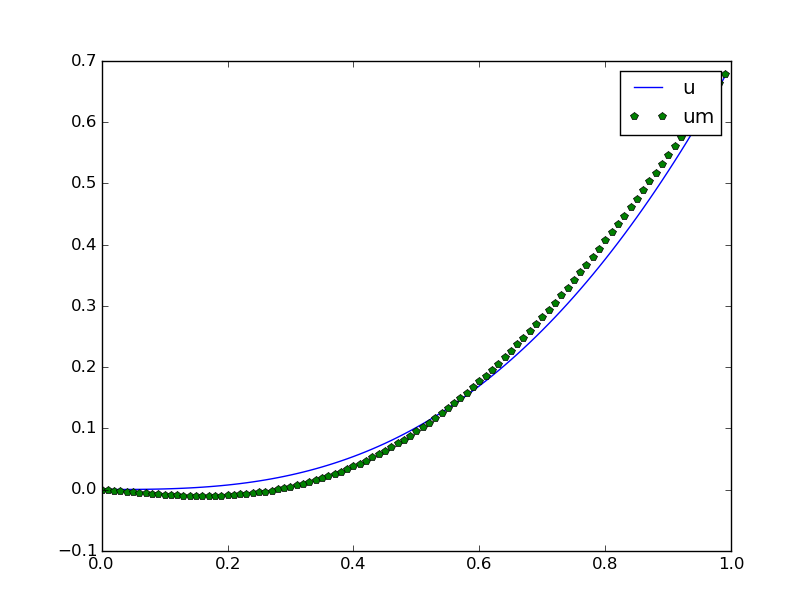
\includegraphics[scale=0.8]{k1.png}
        \caption{Приближение функции $u$ методом аппроксимации Бубнова-Галеркина, при $k = 1$.}
        \label{pic:k1}
    \end{figure}

    \begin{figure}[ht!]
        \centering
        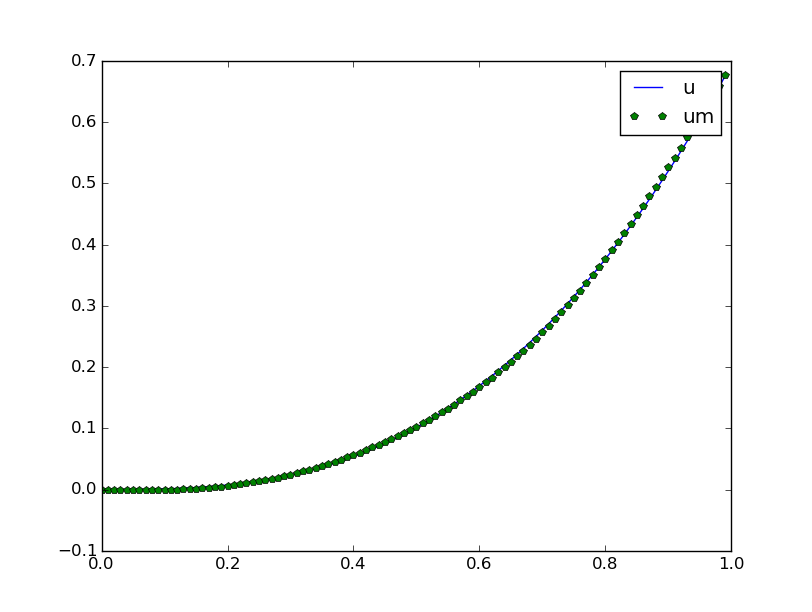
\includegraphics[scale=0.8]{k3.png}
        \caption{Приближение функции $u$ методом аппроксимации Бубнова-Галеркина, при $k = 3$.}
        \label{pic:k3}
    \end{figure}

    \begin{figure}[ht!]
        \centering
        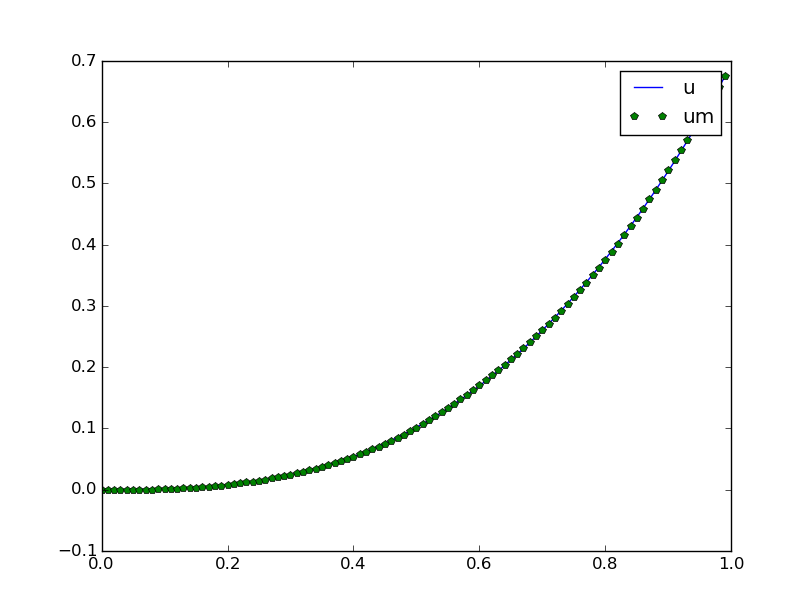
\includegraphics[scale=0.8]{k5.png}
        \caption{Приближение функции $u$ методом аппроксимации Бубнова-Галеркина, при $k = 5$.}
        \label{pic:k5}
    \end{figure}

\end{document}
